% Standalone draft, 2026-11-26; not included in the thesis main file.
\section{共享参数向量场迁移方法}
\label{sec:ch06_shared_vector_field}

第五章利用统计伪配对监督Translator，在独立训练的双域VAE之间学习直接潜变量映射，再由Real Decoder生成目标域触觉。该方法通过GRU内部状态建模四帧序列，但未显式构造潜变量的积分更新路径；配对潜变量误差也不能直接说明Natural Sim输出的域分布是否接近Real。为在保留既有表示与读出模块的条件下研究可调整的迁移路径，本文将原映射扩展为源条件共享参数向量场，通过数值积分获得目标潜状态。这里的扩展是迁移计算形式的改变，并未重新建立公共物理坐标，也不预设两域潜变量具有物理等价性。

记Natural Sim输入为$X_s\in\mathbb R_{\ge0}^{4\times712}$，沿用第五章的记号，以冻结Sim Encoder的后验均值$Z_s=\mu_s(X_s)\in\mathbb R^{4\times64}$作为源条件。积分状态$H(\tau)$同样具有$4\times64$形状，位于Real Decoder接收的潜变量坐标中。与直接令输出等于$T_\theta(Z_s)$不同，向量场同时考虑源条件、当前积分状态和积分坐标，其定义为
\begin{equation}
 \begin{aligned}
 v_\theta(H,Z_s,\tau)&=T_{\theta_T}(Z_s)+c_{\theta_c}(H,Z_s,\tau),\\
 \boldsymbol e(\tau)&=[\tau,1-\tau,\sin(\pi\tau),\cos(\pi\tau)].
 \end{aligned}
 \label{eq:ch06_vector_field}
\end{equation}
其中$T_{\theta_T}$为原Translator初始化的基础映射，$c_{\theta_c}$为状态相关修正项，两者分别具有参数集合$\theta_T$与$\theta_c$，合记为$\theta=(\theta_T,\theta_c)$。共享是指不同Euler步骤复用同一组$\theta$，并非两个子网络的内部权重相同。$\tau\in[0,1]$是归一化计算坐标，不对应机器人运动时间或传感器采样时刻。源条件在每一步均参与计算，积分状态不是在两域潜变量之间直接作线性插值。

修正网络在每个帧位置拼接64维源潜变量、64维当前状态与4维积分坐标特征，形成132维输入，经128维线性投影和GELU后，送入隐藏维数为128的单层GRU，再以线性层输出64维修正。相同$\boldsymbol e(\tau)$广播至窗口内四帧；GRU负责利用帧序列上下文，而积分状态负责承载不同数值步之间的更新。每次向量场调用均重新开始GRU计算，仅沿该次调用的四帧传递循环隐状态，不将其隐状态延续到下一Euler步。该设计将短时序关联与积分推进分开表示，避免把四帧观测误解为四个积分节点。

\begin{samepage}
上述向量场对应的连续状态演化可写为
\begin{equation}
 \frac{\mathrm dH(\tau)}{\mathrm d\tau}
 =v_\theta\bigl(H(\tau),Z_s,\tau\bigr),\qquad
 H(0)=\boldsymbol0_{4\times64},\quad \tau\in[0,1].
 \label{eq:ch06_continuous_state}
\end{equation}
\end{samepage}
该式定义潜状态的计算路径，而非物理动力学。实际实现不求解析解，而以显式Euler法近似该初值问题，部署链路见图\ref{fig:ch06_shared_vector_field}：
\begin{equation}
 \begin{aligned}
 H_0&=\boldsymbol0_{4\times64},\qquad \Delta\tau=K^{-1},\\
 H_{k+1}&=H_k+\frac1K
 v_\theta\!\left(H_k,Z_s,\frac{k}{K}\right),
 \quad k=0,\ldots,K-1,\\
 \widehat X_r&=D_r(H_K).
 \end{aligned}
 \label{eq:ch06_euler_transfer}
\end{equation}
其中$D_r$为冻结的Real Decoder，输出保持完整$4\times712$形状。$K\in\{1,2,4,8\}$控制同一区间的离散步数，全部步骤调用同一个向量场，既不增加独立网络，也不代表增加训练轮次。帧索引$t=1,\ldots,4$与积分索引$k$分别描述观测序列和计算路径；即使二者取值数量相同，也不存在一一物理时间对应。

\begin{figure}[htbp]
 \centering
 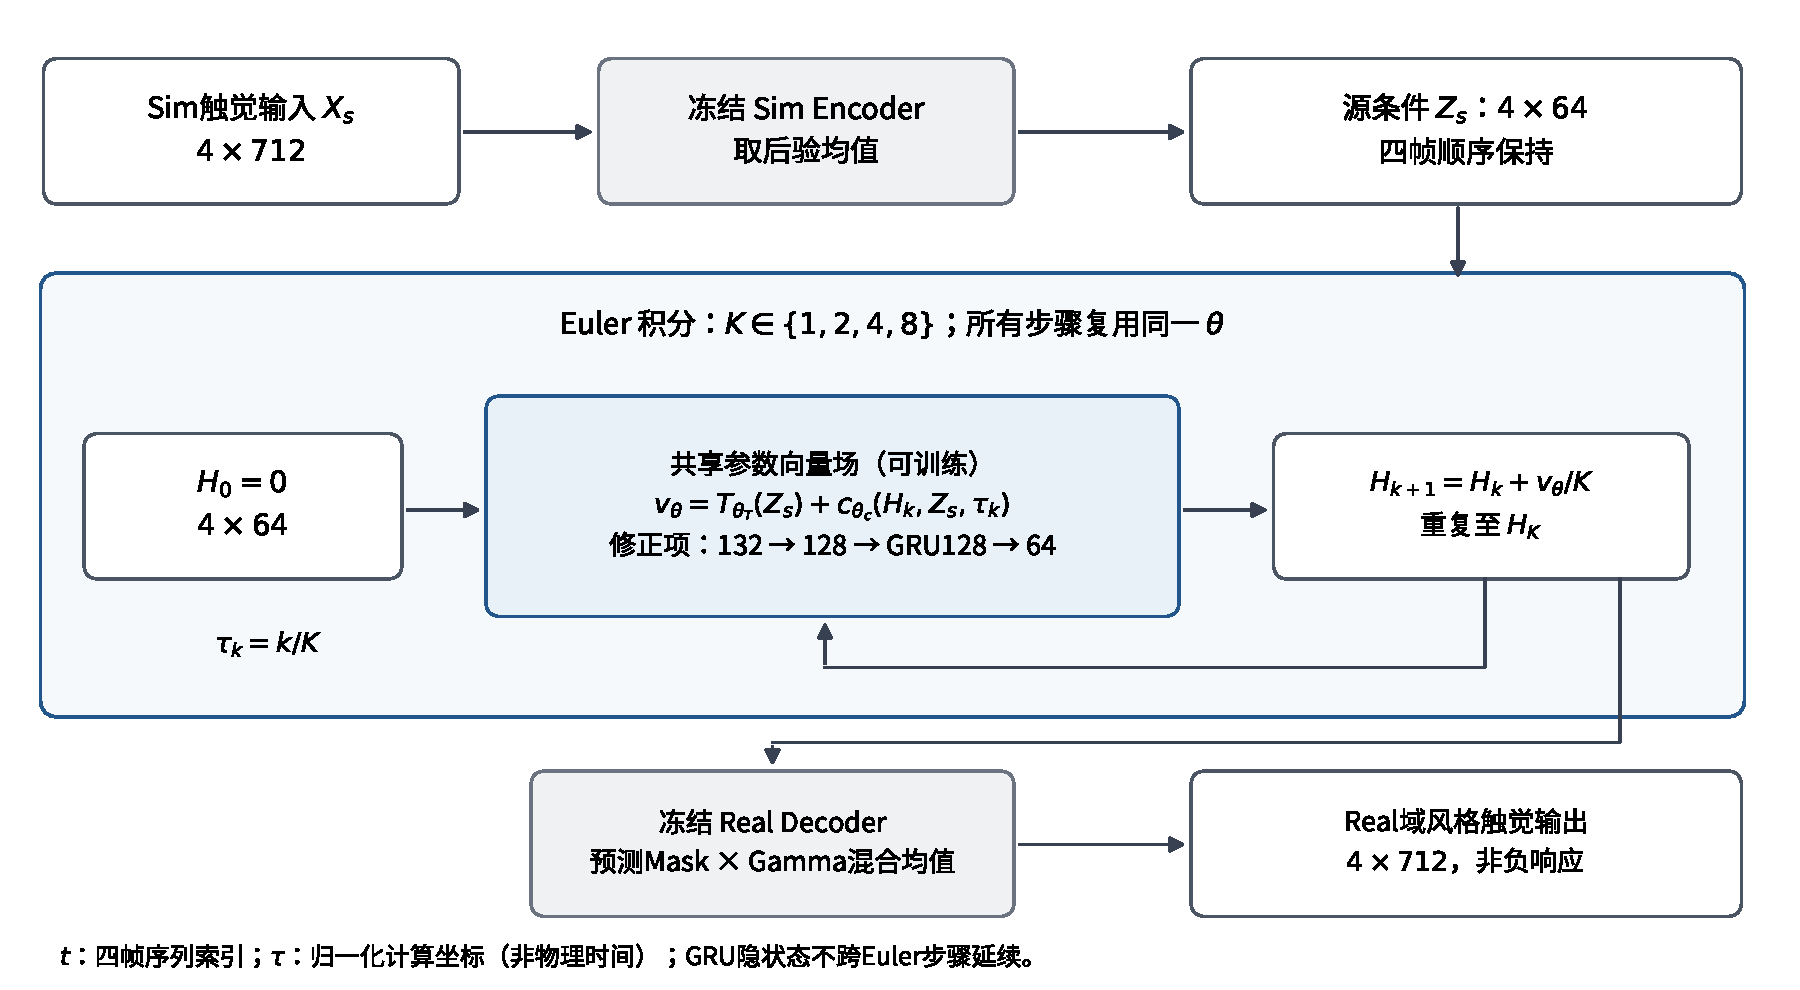
\includegraphics[width=0.98\textwidth,trim=0 4bp 0 26bp,clip]{figures/ch06/shared_vector_field.pdf}
 \caption{共享参数向量场迁移框架。灰色模块冻结，蓝色模块可训练；积分展开复用同一组参数，四帧序列在各次向量场调用内部处理。}
 \label{fig:ch06_shared_vector_field}
\end{figure}

训练时每轮将$[1,2,4,8]$重复16次，以种子4401加轮次初始化的随机数生成器打乱，形成64个批次的步数调度，每种$K$出现16次。前两轮仅预热判别器，随后18轮按相同调度更新同一生成器，而不分别拟合四个模型。这样，不同步数的读出可以在同一组参数下比较，避免将新增网络容量误认为积分细化的作用。对于给定窗口，源后验均值只需编码一次，随后作为固定条件反复传入场；最终仅对积分终点解码。增加步数主要增加场的调用次数，既不增加输入帧数，也不产生新的独立观测。

初始化分别载入原始C3的Real VAE、Sim VAE和Translator权重；后续映射改进版本C27仅参与比较，不作为初始化或教师。修正项末层权重与偏置置零，使初始$c_{\theta_c}$恒为零。因此，在理想数学运算下，任意上述$K$均有$H_K=T_{\theta_T}(Z_s)$，保留原直接映射作为优化起点；实际浮点计算仍需按计算后端检查。这一性质只适用于初始化，修正项随后随训练更新，不受永久零值约束。

完整生成器保留两套VAE及共享向量场，共2494640个参数，其中306176个向量场参数参与更新。可训练部分同时包含Translator基项与修正网络，并非只训练零初始化的末层。两域VAE全部冻结，但冻结Real Decoder仍可向输入潜状态传递梯度。训练目标从第五章的伪配对潜变量监督转向对抗优化、输入保持及修正场幅度约束；初期另使用原C3同源输出的蒸馏项，并逐步降低其权重。该项从首个对抗训练轮的1衰减至第六轮的0，不应将后续无教师项的配置倒填为初始训练合同。具体损失及判别器梯度路径在下一节展开。

\begin{table}[htbp]
 \centering\small
 \caption{直接潜变量映射与共享向量场方法的关系}
 \label{tab:ch06_mapping_comparison}
 \begin{tabular}{p{0.17\textwidth}>{\raggedright\arraybackslash}p{0.32\textwidth}p{0.40\textwidth}}
 \hline
 比较维度 & 第五章直接映射 & 共享参数向量场\\
 \hline
 映射形式 & 直接预测目标潜变量 & 积分更新目标潜状态\\
 映射输入 & Sim后验均值 & Sim后验均值、积分状态及坐标\\
 计算过程 & 一次Translator序列映射 & 同一向量场的Euler积分\\
 训练依据 & 伪配对Huber与条件NLL & 对抗、保持、场约束及初期蒸馏\\
 参数基础 & 双域VAE固定，训练\mbox{Translator} & 继承并冻结双VAE，训练完整场\\
 \hline
 \end{tabular}
\end{table}

表\ref{tab:ch06_mapping_comparison}概括了两种计算形式的关系。最终推理只需Sim Encoder、共享场及Real Decoder，不额外调用原C3教师；Real Encoder和Sim Decoder虽保留在完整模型中，也不位于部署链路。Decoder采用预测Mask与恢复尺度的Gamma混合均值输出非负响应。由此得到的是Real域风格触觉，而非已认证的真实接触测量。共享场提供了在既有潜表示上修正迁移路径的机制，但增加积分步数是否改善分布及输入保持，仍须由后续实验判断，不能由框架本身推导出迁移成功。
